% Chapter 5

\chapter{Drawings} % Main chapter title

\label{Chapter4} % For referencing the chapter elsewhere, use \ref{Chapter1} 

\lhead{Chapter 4. \emph{Drawings}} % This is for the header on each page - perhaps a shortened title

%----------------------------------------------------------------------------------------
\begin{figure}[htbp]
	\centering
		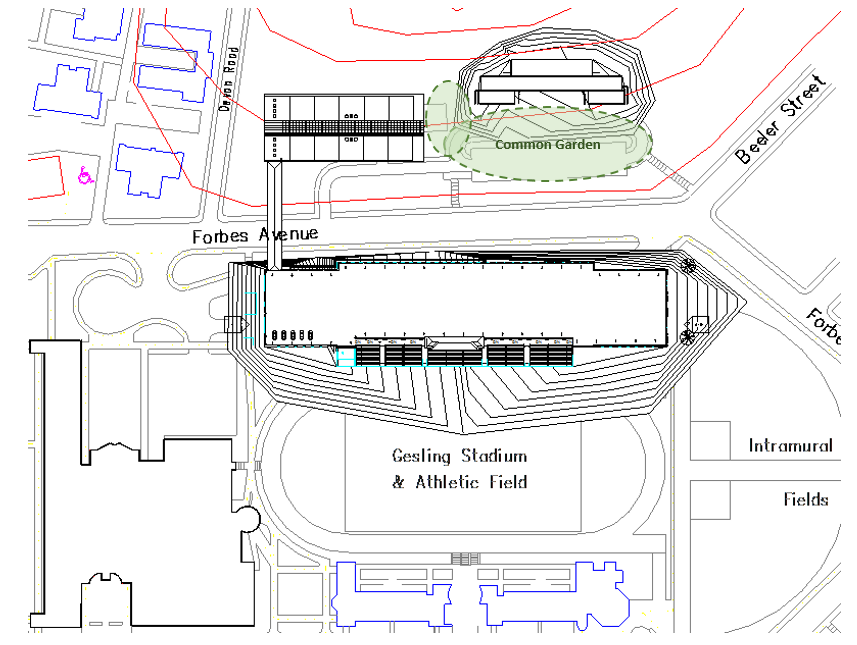
\includegraphics[width=\textwidth]{sitePlan.png}
	\caption[Site Plan]{Site Plan}
	\label{fig:sitePlan}
\end{figure}

\begin{figure}
\centering
\begin{subfigure}{0.5\textwidth}
  \centering
  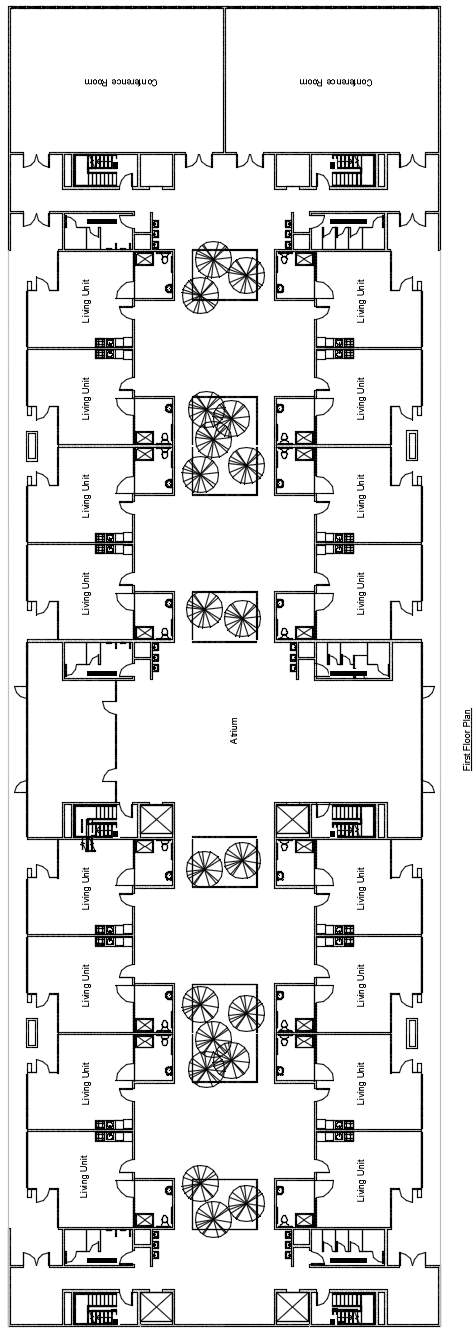
\includegraphics[width=\linewidth]{FirstFloorPlan.png}
  \caption{First Floor Plan}
  \label{fig:FirstFloorPlan}
\end{subfigure}%
~
\begin{subfigure}{0.5\textwidth}
  \centering
  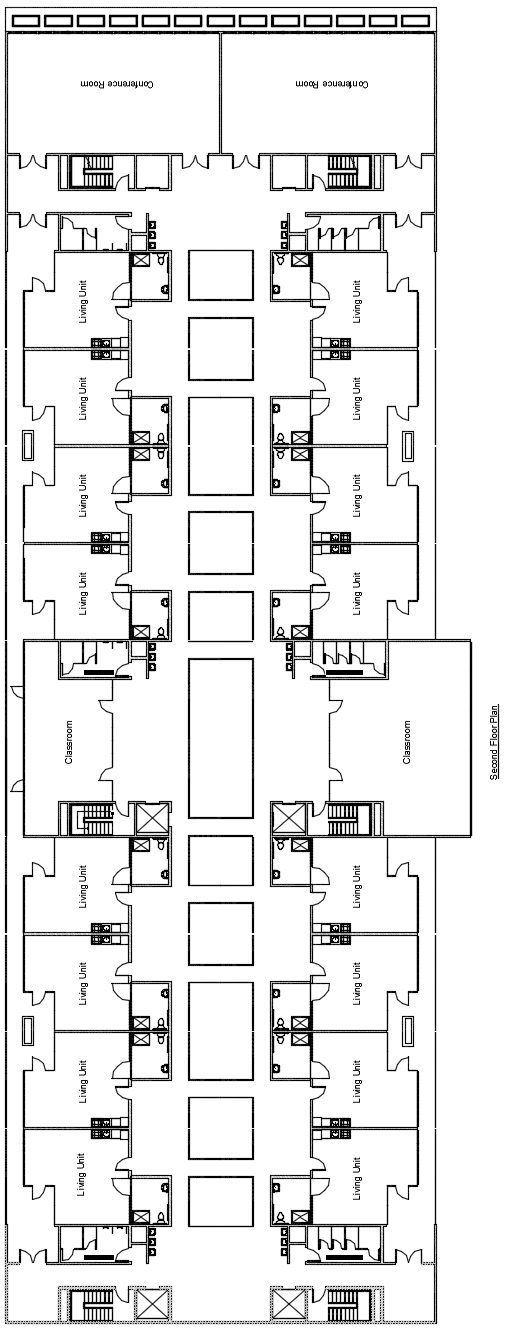
\includegraphics[width=\linewidth]{SecondFloorPlan.png}
  \caption{Second Floor Plan}
  \label{fig:SecondFloorPlan}
\end{subfigure}
\caption{FloorPlan, First Floor and Second Floor}
\label{fig:FloorPlan-Level1-2}
\end{figure}

\begin{figure}
\centering
\begin{subfigure}{0.5\textwidth}
  \centering
  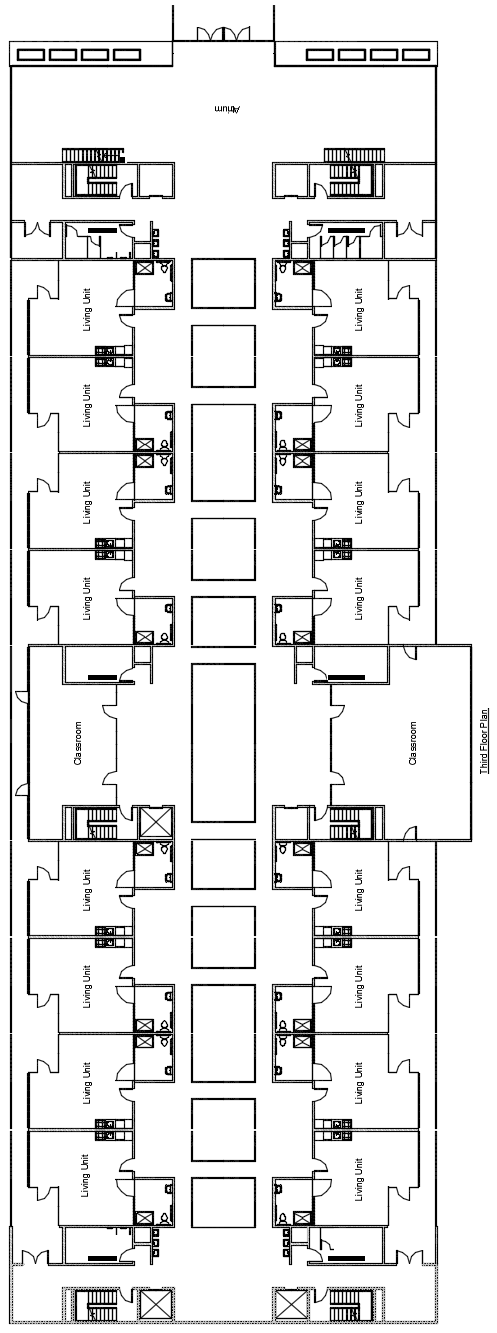
\includegraphics[width=\linewidth]{ThirdFloorPlan.png}
  \caption{Third Floor Plan}
  \label{fig:ThirdFloorPlan}
\end{subfigure}%
~
\begin{subfigure}{0.5\textwidth}
  \centering
  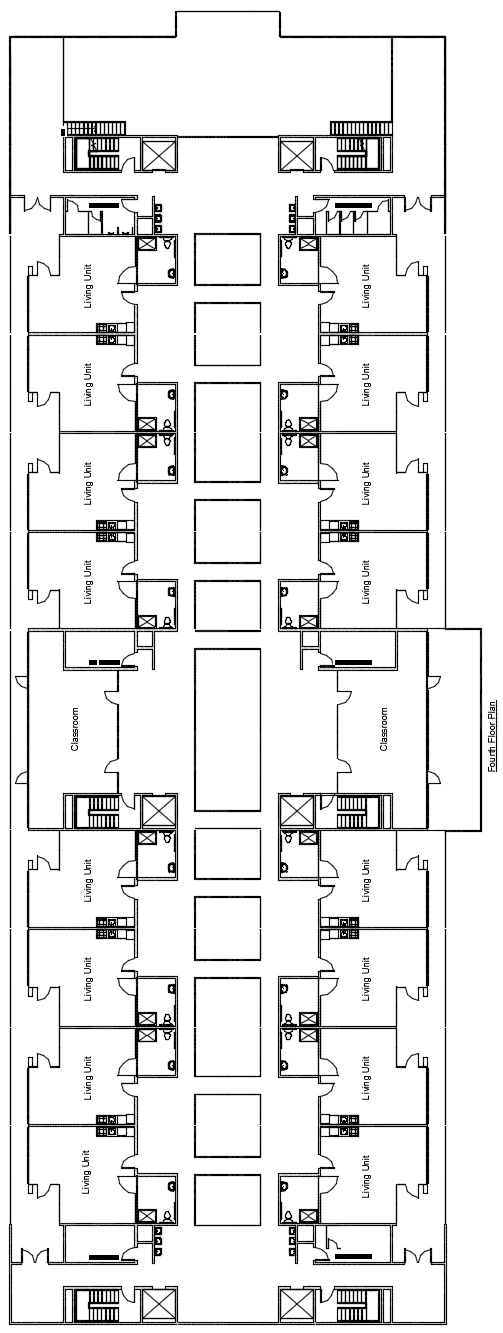
\includegraphics[width=\linewidth]{FourthFloorPlan.png}
  \caption{Fourth Floor Plan}
  \label{fig:FourthFloorPlan}
\end{subfigure}
\caption{FloorPlan, Third Floor and Fourth Floor}
\label{fig:FloorPlan-Level3-4}
\end{figure}

\begin{figure}[t!]
\centering
\begin{subfigure}{0.5\textwidth}
  \centering
  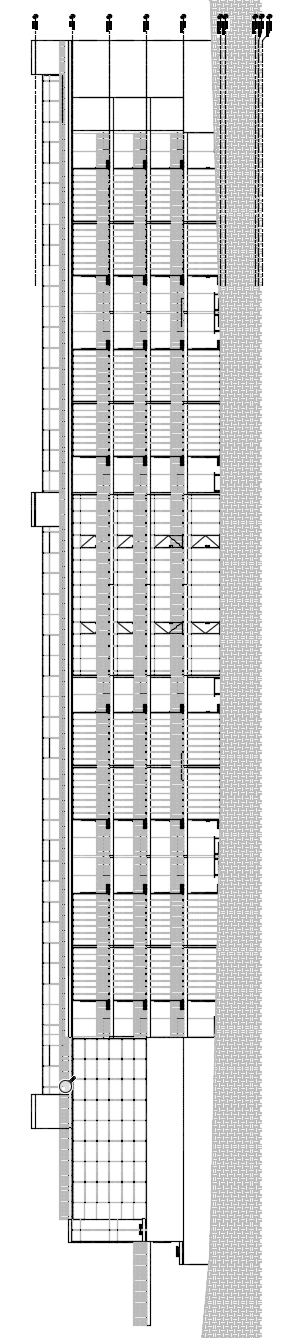
\includegraphics[height = 9in]{ElevationNorth.png}
  \caption{Elevation North}
  \label{fig:ElevationNorth}
\end{subfigure}%
~
\begin{subfigure}{0.5\textwidth}
  \centering
  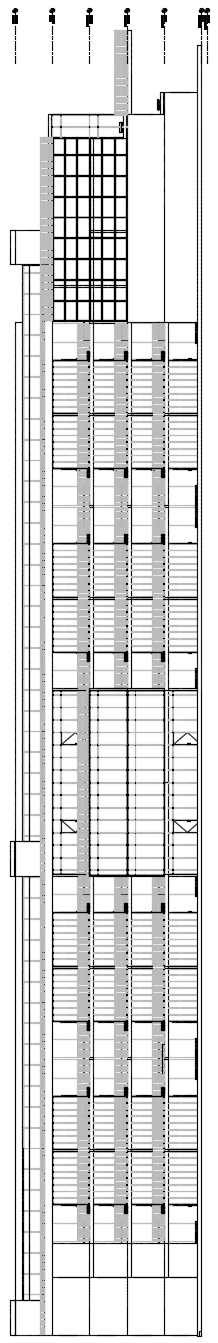
\includegraphics[height = 9in]{ElevationSouth.png}
  \caption{Elevation South}
  \label{fig:ElevationSouth}
\end{subfigure}
\caption{Elevation, North and South}
\label{fig:ElevationNS}
\end{figure}

\begin{figure}[t!]
\centering
\begin{subfigure}{\textwidth}
  \centering
  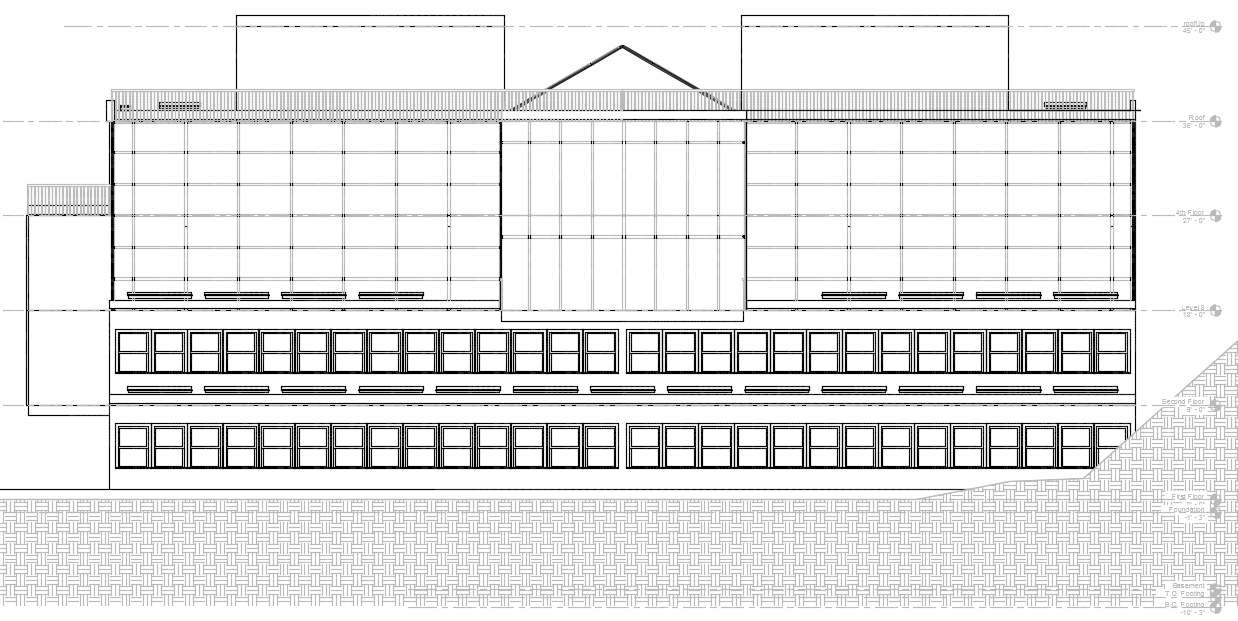
\includegraphics[width = \linewidth]{ElevationEast.png}
  \caption{Elevation East}
  \label{fig:ElevationEast}
\end{subfigure}

\begin{subfigure}{\textwidth}
  \centering
  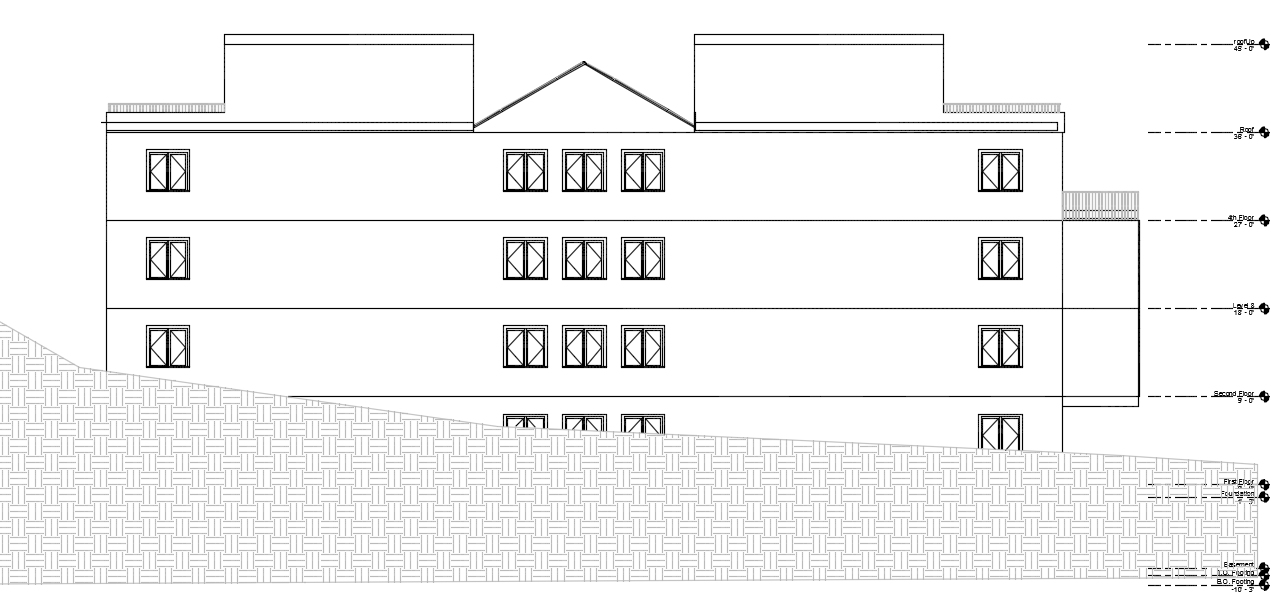
\includegraphics[width = \linewidth]{ElevationWest.png}
  \caption{Elevation West}
  \label{fig:ElevationWest}
\end{subfigure}
\caption{Elevation, East and West}
\label{fig:ElevationEW}
\end{figure}